
\begin{center}
\Huge
Monotonisætningen og monotoniforhold
\end{center}
\section*{Monotonisætningen}
\stepcounter{section}
Hvis en funktion aftager efter et toppunkt og funktionen ikke har flere ekstremumspunkter til højre for dette toppunkt, så virker det intuitivt at funktionen bliver ved med at aftage efter toppunktet. Dette gælder også tilsvarende for voksende funktioner og minima. Vi har en sætning, der præciserer denne idé for differentiable funktioner. Denne kalder vi for monotonisætningen. 
\begin{setn}[Monotonisætningen]
Lad $f$ være differentiabel på et interval $I$. Så gælder der følgende:
\begin{enumerate}[label=\roman*)]
\item Hvis $f'(x)>0$ for alle $x$ i intervallet $I$, så vil $f$ være voksende på $I$.
\item Hvis $f'(x)<0$ for alle $x$ i intervallet $I$, så vil $f$ være aftagende på $I$. 
\item Hvis $f'(x)=0$ for alle $x$ i intervallet $I$, så er $f$ konstant på $I$.
\end{enumerate}
\end{setn}
Det er ikke svært at bevise monotonisætningen, men det er derimod en smule omfattende. 

Vi skal hovedsagligt bruge monotonisætningen til at bestemme monotoniforhold for differentiable funktioner. Vi skal altså afgøre på hvilke intervaller funktioner er monotone. Lad os betragte et eksempel.
\begin{exa}
Vi ønsker at bestemme monotoniforholdene for funktionen $f(x) =\frac{1}{3}x^3-\frac{1}{2}x^2-2x$. Vi starter med at plotte $f$ som kan ses af Fig. \ref{fig:monof}.

\begin{figure}[H]
\centering
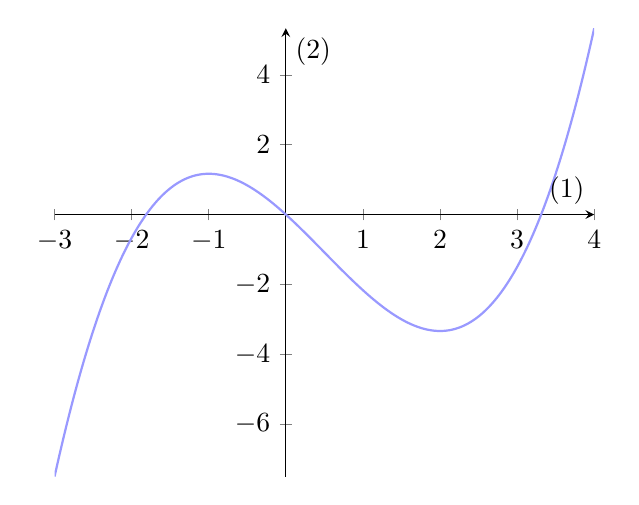
\begin{tikzpicture}
\begin{axis}[axis lines=middle,
xlabel = (1),
ylabel = (2)]
\addplot[color=blue!40,thick, domain=-3:4, samples=1000]{1/3*x^3-1/2*x^2-2*x};
\end{axis}
\end{tikzpicture}
\caption{Plot af funktionen $f$}
\label{fig:monof}
\end{figure}
For at finde monotoniforholdene for $f$ starter vi med at differentiere $f$ for at se, hvor $f$ har ekstremumspunkter. Vi finder derfor $f'(x) = x^2-x-2$ og sætter denne lig nul:
\begin{align*}
f'(x)=x^2-x-2 = 0,
\end{align*}
som har løsningerne $x=-1$ og $x=2$. Funktionen $f$ har derfor ekstremumspunkter i $x=-1$ og $x=2$. Vi bruger $f'$ til at afgøre, hvornår $f$ er voksende og aftagende ved at indsætte et tal på $x$ plads mellem $-1$ og $2$, et tal mindre end $-1$ og et tal større end $2$. Derfor får vi
\begin{align*}
f'(-2) = (-2)^2+2-2 = 4, 
\end{align*} 
og monotonisætningen siger derfor, at $f$ vokser på intervallet $]-\infty,-1]$. 
\begin{align*}
f'(0) = 0^2-0-2 = -2,
\end{align*}
og monotonisætningen siger derfor, at $f$ aftager på intervallet $[-1,2]$.
\[ 
f(3) = 3^2-3-2 = 9-5=4,
\]
og monotonisætningen siger derfor, at $f$ vokser på intervallet $[2,\infty[.$
Vi opskriver desuden en monotonilinje
\begin{center}
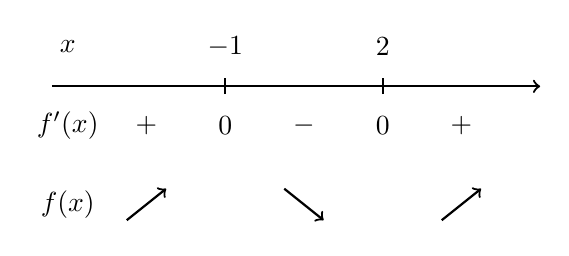
\begin{tikzpicture}
\node at (0,0) {$x$};
\node at (0,-1) {$f'(x)$};
\node at (0,-2) {$f(x)$};
\node at (2,0) {$-1$};
\node at (4,0) {$2$};
\node at (2,-1) {0};
\node at (4,-1) {0};
\node at (1,-1) {$+$};
\node at (3,-1) {$-$};
\node at (5,-1) {$+$};
\draw[->,thick] (-0.2,-0.5) to (6,-0.5);
\draw[thick] (2,-0.6) to (2,-0.4);
\draw[thick] (4,-0.6) to (4,-0.4);
\draw[->,thick] (0.75,-2.2) to (1.25,-1.8);
\draw[->,thick] (2+0.75,-1.8) to (2+1.25,-2.2);
\draw[->,thick] (4+0.75,-2.2) to (4+1.25,-1.8);
\end{tikzpicture}
\end{center}
Bemærk, at vi i princippet ikke behøver grafen for funktionen for at bestemme monotoniforholdene. 
\end{exa}
\section*{Opgave 1}
Bestem monotoniforholdene for følgende funktioner (Bemærk, at vi ikke kan vælge hele $\mathbb{R}$ som definitionsmængde for alle funktionerne)
\begin{align*}
&1) \ x^2   &&2)\ 3x^3-10  \\
&3) \ x+10  &&4)\ x^4 \\
&5) \ \sqrt{x}+x^2  &&6)\ \frac{1}{x} -x^2 \\
&7) \ \sin(x)  &&8)\ \cos(x)  